% Chapter Template

\chapter{Angular} % Main chapter title

\label{Chapter4} % Change 4 to a consecutive number; for referencing this chapter elsewhere, use \ref{Chapter4}

\section{Definition}

Angular is a JavaScript framework for developing client side applications. This framework was created on October 2010 by Google. It is maintained by Google and a community of individual developers since September 2016 that its code became open source. (\cite{Reference6}) Angular as framework is providing a large set of libraries, functions and tools, and its implementing the entire structure of a client-side application. Moreover, Angular is using templates that extend HTML style syntax for view's representation, and is built in TypeScript, a JavaScript-like language. (\cite{Reference19}) \par

Angular's advantage is that provides the ability of creating and managing project through terminal. Due to its complicated set up, Google created a command line interface, or CLI, that makes Angular's usage much easier. Angular CLI is responsible for creating and maintaining common pattern inside an app. (\cite{angularUpandRunning}) Creating projects, adding new controllers and much more other tasks, are automated and easy implemented with just one command. Last but not least, Angular CLI is based on Webpack, a tool that groups TypeScript, JS, CSS, HTML and any files used in the application, and makes deployment, building app for production, simpler. (\cite{murray2018ng}) \par

\subsection{Angular \& AngularJS}

AngularJS, or sometimes referred as Angular 1, was firstly released in order to provide quick, scalable and maintainable web applications. As years passed, the way browsers, and generally web, used to work changed dramatically, so AngularJS stopped solving problems relevant with the new updates of web. Thus, Angular was created on 2014 which is basically a totally newly written framework. As "Angular" are referred all the newest version, starting from Angular2 and above.(\cite{angularUpandRunning}) \par

More specifically, Angular and AngularJS are two different frameworks made from the same team. As regards AngularJS, it is using directives, controllers, scopes, services and dependency injections, while Angular is using components, instead of directives, and services. Comparing these two frameworks, modules were replaced by web components and existing features of AngularJS were improved, such as dependency injection and templating. (\cite{angularUpandRunning}) Scope, which stands for two-way binding, and directive definition objects, controllers and angular.module were removed from the new versions of Angular. (\cite{murray2018ng}) \par

\subsection{HTTP}

Angular is providing an impended HTTP library through which external APIs can be called. The HTTP requests made are asynchronous that enhance pages performance. This means that user can continue interacting without waiting for the HTTP's response. In general, there are three ways of dealing with asynchronous code in Angular, Callbacks, Promises and Observables. (\cite{murray2018ng})

\section{Typescript}

\begin{wrapfigure}[12]{r}{0.3\textwidth}
	\begin{center}
		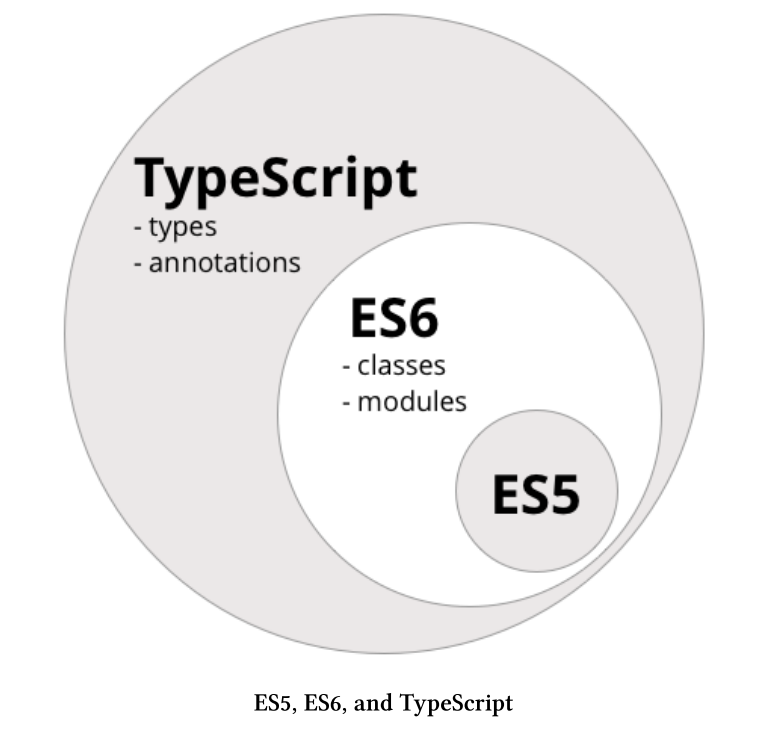
\includegraphics[scale=0.25]{images/Typescript.png}
	\end{center}
	\caption{Typescript}
\end{wrapfigure}

Angular is using a JavaScript-based language named TypeScript, which was the result of Microsoft's and Google's collaboration. TypeScript is a superset of ES6 with the additional features of types and annotations, as it is shown in the diagram bellow, and is compiled to ES5 in order code to be compatible with browsers. (\cite{murray2018ng}) \par

It is not obligatory to write TypeScript in Angular apps.However, it is a good practice due to the features provided, that also make coding easier to be maintained and understood. (\cite{angularUpandRunning}) \par

\subsection{Types}

TypeScript's name was inspired by its typing system, the most important addition to its ES6 code. Type checking can prevent developers from bugs and make code much readable due to its obligatory clarification. (\cite{murray2018ng}) \par 

Regarding types provided, they are the same as in JavaScript, booleans (true or false), numbers, strings, arrays, enums (similar to arrays but has numeric values as names), any (any type of value), void (no type or returned value expected). Types are not necessarily used in TypeScript, they can be omitted in case of wanting to write quick code. (\cite{murray2018ng}) \par

\subsection{classes} 


\subsection{utilities}  (e.g. destructuring)


\section{Components} %maybe?


\section{LifeCycle Methods}


\section{Two or one-way data binding}

Two-way data binding is an architecture in which information flows from state to view and vice versa. In Angular JS, the default data flow is the two-way binding, or MVW as noticed in \ref{Chapter2}, which means that when model is modified, view is also changed and the other way around. (\cite{murray2018ng}) This type of binding is easy to start with and is also suitable for totally interactive user interfaces since data are changed by two different directions. (\cite{Reference21}) \par

On the other hand, two direction data binding is possible to cause a flow of unpredictable updates and a difficulty to follow data flow as application goes bigger. Moreover, another problem with this architectural approach is that it binds data flow with DOM tree. For these reasons, new released Angular is flexible to change between one or two-way data structure if it is needed. As described in Chapter \ref{Chapter2}, two-direction binding pass data down via components and event handlers needed to reflect state based on view layer's changes. For adapting one-way structure, Angular can use either Observables-based, such as Reactive Extensions Library for JavaScript (RxJS), or Flux-based architecture, such as Redux. When using Observables as main data architecture in Angular, it is named Reacting Programming which is a way to use asynchronous data streams. (\cite{murray2018ng}) \par

\section{Summery}


% 6 pages
